%% This is an example first chapter.  You should put chapter/appendix that you
%% write into a separate file, and add a line \include{yourfilename} to
%% main.tex, where `yourfilename.tex' is the name of the chapter/appendix file.
%% You can process specific files by typing their names in at the 
%% \files=
%% prompt when you run the file main.tex through LaTeX.

\begingroup%
\makeatletter%
\cleardoublepage%
\let\newpage\relax%
\let\clearpage\relax%
\vspace*{\fill}%
\vspace*{\dimexpr-50\p@-\baselineskip}% Remove the initial
%% -default- 50pt gap (plus 1 line) 
\chapter[Supporting information for Chapter 2]{{\setlength{\huge} Supporting information for}\\ \autoref{chap2}: Multiple Fates of Sinking Particles in the North Atlantic Ocean}
\label{AppC}
\let\thefootnote\relax\footnote{{\setlength{\parindent}{0pt}This supporting information was originally published in conjunction with:\\\\Collins, J. R., B. R. Edwards, K. Thamatrakoln, J. E. Ossolinski, G. R. DiTullio, K. D. Bidle, S. C. Doney, and B. A. S. Van Mooy. 2015. The multiple fates of sinking particles in the North Atlantic Ocean. \emph{Global Biogeochemical Cycles} \emph{29}:1471-1494; doi:\href{http://dx.doi.org/10.1002/2014GB005037}{10.1002/2014GB005037}\\\\\copyright 2015 American Geophysical Union}}
\vspace*{\fill}%
\endgroup%

\clearpage

\section{Supplementary Figures}

\begin{figure}[!th]
\centering
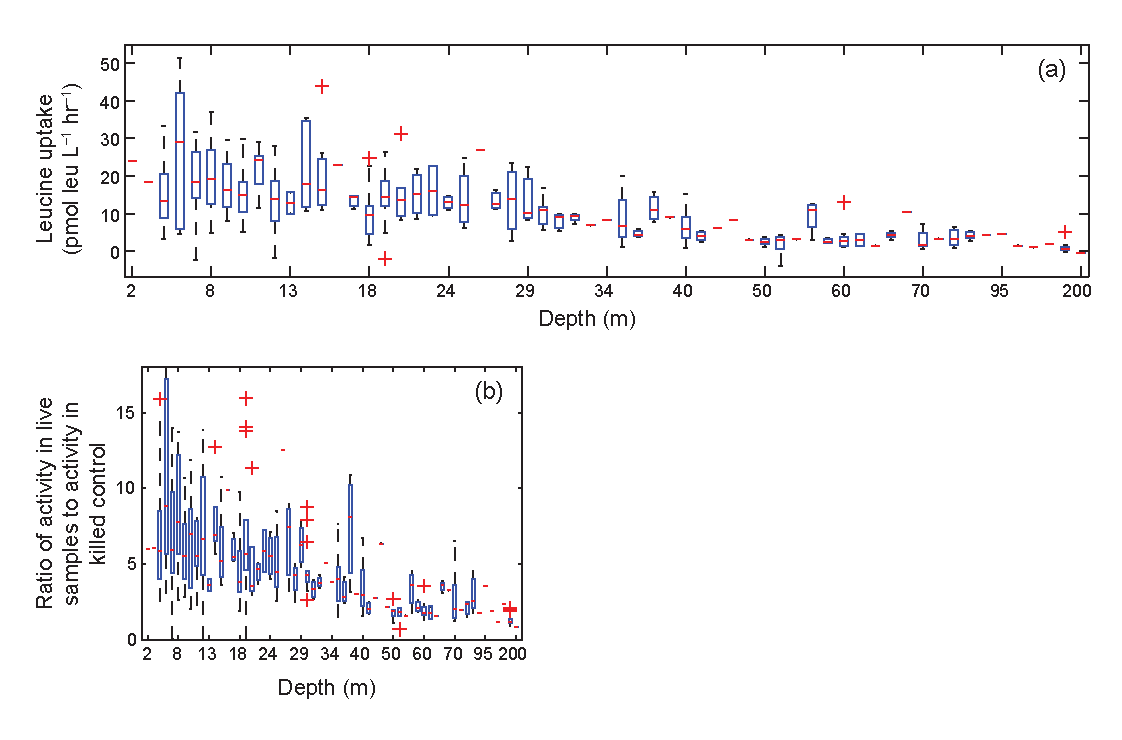
\includegraphics[width=1\textwidth]{Fig_C-1.pdf}
\captionsetup{font={footnotesize}}
\caption[Summary statistics for bacterial production data]{Summary statistics for bacterial production data. (a) Box-and-whisker plot by depth of all leucine incorporation observations, corrected for activities in killed control samples. (b) Box-and-whisker plot by depth of the signal-to-noise ratio, i.e., the ratio of the mean of the activity measured in the three live replicates to the activity in the killed control. Red lines represent the median values for each depth, box extremities are the 75\textsuperscript{th} and 25\textsuperscript{th} quartiles, whisker tails are 95\textsuperscript{th} and 5\textsuperscript{th} quartiles, and red + symbols represent outliers.
}
\label{fig:acn1}
\end{figure}

\clearpage

\begin{figure}[!th]
\centering
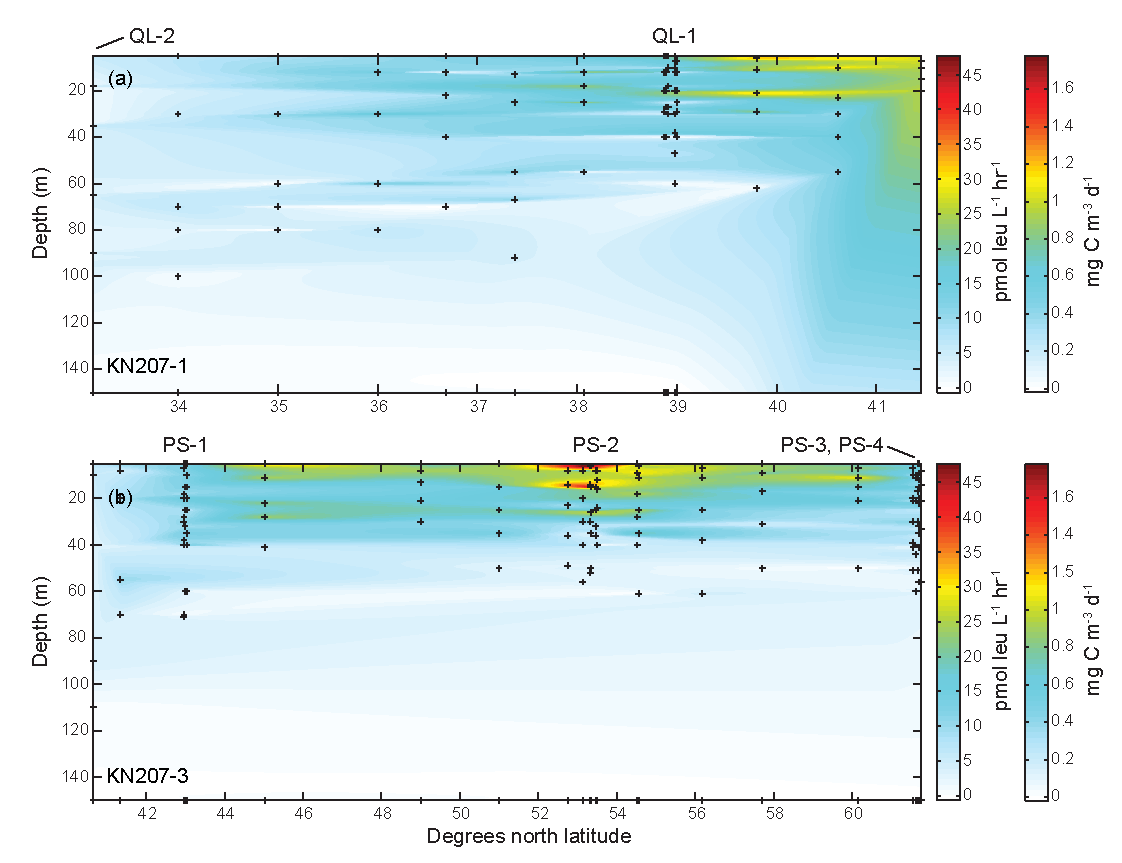
\includegraphics[width=1\textwidth]{Fig_C-2.pdf}
\captionsetup{font={footnotesize}}
\caption[Contour plots of water column bacterial production rates along the KN207-1 and KN207-3 cruise tracks]{Contour plots of water column bacterial production rates measured using the \textsuperscript{3}H-leucine incorporation method along the (a) KN207-1 and (b) KN207-3 cruise tracks. Data are presented in volumetric units of leucine uptake and in mg C m\textsuperscript{-3} d\textsuperscript{-1}. For conversion to units of C in these plots (on secondary axis), an isotope dilution (\emph{ID}) of 1 and a conversion factor ${\nu _{C:leu}}$ of 1.5 kg C (mol leu)\textsuperscript{-1} were assumed, making the rates a minimum estimate of bacterial carbon turnover. Superimposed (+) are locations of our discrete observations, which we used to generate the contour plots. Also superimposed are the locations of the six process stations.
}
\label{fig:acn2}
\end{figure}

\clearpage

\begin{figure}[!th]
\centering
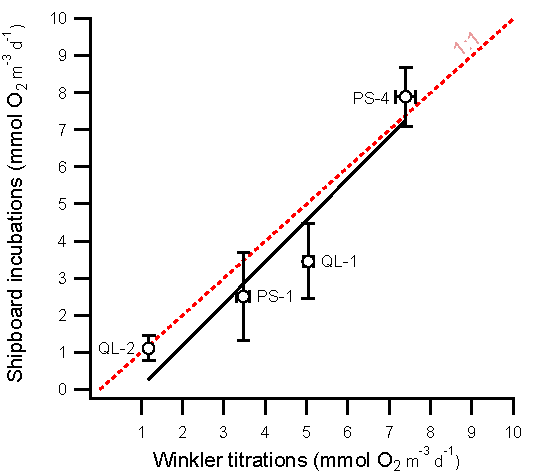
\includegraphics[width=0.5\textwidth]{Fig_C-3.pdf}
\captionsetup{font={footnotesize}}
\caption[Mixed layer community respiration rates at four process stations calculated using two different methods]{Mixed layer community respiration rates at four process stations calculated using two different methods. \emph{x}-axis: Rates calculated from a series of 300 mL shipboard incubations using optode sensor spots. \emph{y}-axis: Rates calculated using a traditional two-point Winkler titration method. A type II (major axis---orthogonal distance) linear regression was fit to the data (solid black trace; $y = 1.13x - 1.07$; r\textsuperscript{2} = 0.95). A 1:1 line (dashed red trace) is superimposed for reference. Error bars represent uncertainties from replication (Winkler method) or the standard error of regression (incubations).
}
\label{fig:acn3}
\end{figure}

\clearpage

\section{Supplementary Tables}

\clearpage

\begin{landscape}
\begin{scriptsize}
\begin{singlespace}
\begin{flushleft}
%\renewcommand*{\arraystretch}{1.3}
\begin{longtable}{ Lp{.29\linewidth} Lp{.08\linewidth} Lp{.09\linewidth} Lp{.05\linewidth} Lp{.25\linewidth} Lp{.15\linewidth} }
\captionsetup{font={normalsize}}
\caption[Microbial Metabolic Demand and Partitioning between Processes Responsible for Particle Flux Attenuation]{Depth-Integrated Measures of Microbial Metabolic Demand and Model-Diagnosed Estimates of the Partitioning between Major Processes Responsible for Particle Flux Attenuation}
\label{table:acn1}
\endfirsthead
\endhead
\toprule
Location & Depth or depth range for which reported (m) & Average particle sinking velocities (\emph{W\textsubscript{avg}}; m d$^{-1}$) & No. individual observations (\emph{N}) tabulated & Notes & Reference \\
\midrule
Bermuda-Atlantic Time Series (BATS) study site, Sargasso Sea (31$^{\circ}$ $40'$ N, 64$^{\circ}$ $10'$ W) & 150-500 & 13-70 & 4 & Individual observations & McDonnell et al. (2015) \\

Porcupine Abyssal Plain (PAP) site (48$^{\circ}$ N, 16.5$^{\circ}$ W) & 50-500 & 30-250 & 29 & Individual observations; only one observation \textgreater 200 m d$^{-1}$ & Villa-Alfageme et al. (2014) \\

Multiple sites along E-W cruise transect from Massachusetts to NW Africa, & 0-500 & 0.2-22 & 22 & Individual observations for lithogenic particles from Aeolian inputs & Ohnemus and Lam (2014) \\

PAP site & 50 & 9 $\pm$ 9 & --- & Mean for slow sinking particle size pool (\textless 10 m d$^{-1}$) & Riley et al. (2012) \\
 &  & 181 $\pm$ 8 & --- & Mean for fast sinking pool (\textgreater 350 m d$^{-1}$) &  \\

Coastal Norway (60$^{\circ}$ $16'$ N, 5$^{\circ}$ $12'$ E) &  & 9 & --- & Mean value for all sediment trap material between 80-400 $\mu$m & Bach et al. (2012) \\

 &  & 12.5 $\pm$ 4.8 & --- & Mean value for fecal pellets &  \\

Canary Current (27$^{\circ}$ $30'$ N, 016$^{\circ}$ $15'$ W; 27$^{\circ}$ $30'$ N, 15$^{\circ}$ $45'$ W) & 260 & 0.7-11 & --- & Range given for slow-sinking particle fraction comprising  $\sim$ 60\% of total POC & Alonso-Gonz\'{a}lez et al. (2010) \\

POMME study area, NE of Azores (39-45$^{\circ}$ N, 15-21$^{\circ}$ W ) & \textless 1000 m & 10 & --- & Mean value estimated for particle size fraction \textgreater 100 $\mu$m diameter; largely based on observations in mesoscale eddy features & Guidi et al. (2007) \\

N-S JGOFS cruise transect from NW of Azores (40$^{\circ}$ $37'$ N, 20$^{\circ}$ $5'$ W) to Iceland (63$^{\circ}$ $1'$ N, 22$^{\circ}$ $25'$ W) & \textless 1025 m & 137.8-162.5 & --- & Lower and upper limits for bulk sinking particle material from coccolithophore blooms & Knappertsbusch and Brummer (1995) \\

 &  & 123-156 with $\bar x = 141$ $\pm$ 11& 6 & Estimates for particles from individual coccolithophore species &  \\

NABE site W of Madeira Island (34$^{\circ}$ N, 21$^{\circ}$ W) & \textless 1000 m & 46 & 1 & Individual observation & Honjo and Manganini (1993) \\

NABE site in central N. Atlantic (48$^{\circ}$ N, 21$^{\circ}$ W) & \textless 1000 m & 32-116 & 3 & Individual observations & Honjo and Manganini (1993) \\

Porcupine Seabight (50$^{\circ}$ N, 13$^{\circ}$ W) & Surface to deep ocean & 100-150 & --- & Range of values for diatom aggregates & Billett et al. (1983) \\
\bottomrule
\captionsetup{font={footnotesize}}
\caption*{\textsuperscript{a} We restricted our reporting of the literature to values measured for depths \textless{} 1000 m for the region between 22$^{\circ}$ N and 66$^{\circ}$ N latitude. From these 9 studies, we gathered 72 individual observations of the average particle sinking velocity; these were used to generate the histogram in \autoref{fig:c2n5}s. Where values were reported for multiple depth ranges, we used the observations most applicable to the range of depths (50-300 m) we evaluated in our study. An extensive compilation of sinking speed data for Atlantic tropical systems (Cape Blanc, E. and W. Equatorial Atlantic, Benguela Current) and the Southern Ocean can be found in Fischer and Karakas (2009).}
\end{longtable}
\end{flushleft}
\end{singlespace}
\end{scriptsize}

\clearpage

\begin{scriptsize}
\begin{singlespace}
\begin{flushleft}
%\renewcommand*{\arraystretch}{1.3}
\begin{longtable}{ Lp{.055\linewidth} Lp{.04\linewidth} Lp{.10\linewidth} Lp{.12\linewidth} Lp{.07\linewidth} Lp{.07\linewidth} Lp{.08\linewidth} Lp{.08\linewidth} Lp{.02\linewidth} Lp{.08\linewidth}  Lp{.08\linewidth}}
\captionsetup{font={normalsize}}
\caption[Water Column Respiration Rates Measured in the Mixed Layer Using Two Methods]{Water Column Respiration Rates Measured in the Mixed Layer Using Two Methods, April-July 2012\textsuperscript{a}}
\label{table:acn2}
\endfirsthead
\endhead
\toprule
Cruise & Station & Location & Deployment Dates & Euphotic Zone Depth\textsuperscript{b} (m) & Depth of Observation (m) & \multicolumn{2}{ p{.16\linewidth}}{Respiration Rate\textsuperscript{c} (mmol O$_2$ m$^{-3}$ d$^{-1}$ $\pm$ uncertainty)} &  & \multicolumn{2}{ p{.16\linewidth}}{Method Precision (error as \% of rate estimate)} \\
\cmidrule{7-8}
\cmidrule{10-11}
 &  &  &  &  & & Shipboard Incubations\textsuperscript{d} & Winkler Titrations\textsuperscript{e} & & Shipboard Incubations & Winkler Titrations  \\
\midrule
KN207-1 & QL-1 & 38$^{\circ}$ $52'$ $47.4''$ N 69$^{\circ}$ $6'$ $19.2''$ W & 24-27 Apr 2012 & 38 & 29 & 3.46 $\pm$ 1.01 & 5.04 $\pm$ 0.12 &  & 29.20\% & 2.39\% \\

 & QL-2 & 32$^{\circ}$ $57'$ $2.4''$ N 65$^{\circ}$ $44'$ $58.8''$ W & 30 Apr-3 May 2012 & --- & 14 & 1.11 $\pm$ 0.34 & 1.18 $\pm$ 0.04 &  & 30.60\% & 3.39\% \\

KN207-3 & PS-1 & 43$^{\circ}$ $1'$ $58.6''$ N 27$^{\circ}$ $15'$ $31.8''$ W & 17-19 Jun 2012 & 58 & 20 & 2.51 $\pm$ 1.18 & 3.47 $\pm$ 0.16 &  & 47.00\% & 4.73\% \\

 & PS-2 & 53$^{\circ}$ $29'$ $43.0''$ N 30$^{\circ}$ $45'$ $2.6''$ W & 23-27 Jun 2012 & 26 & 7 & 4.03 $\pm$ 0.46 & --- &  & 11.40\% & --- \\

 & PS-3 & 61$^{\circ}$ $37'$ $9.22''$ N 34$^{\circ}$ $6'$ $9.64''$ W & 1-5 Jul 2012 & 42 & 21.5 & 2.55 $\pm$ 1.11 & --- &  & 43.50\%  & --- \\

 &  &  &  &  &  &  &  &  &  &  \\

 & PS-4 & 61$^{\circ}$ $41'$ $40.4''$ N 33$^{\circ}$ $46'$ $21.7''$ W & 7-11 Jul 2012 & 41 & 20 & 7.90 $\pm$ 0.80 & 7.40 $\pm$ 0.23 &  & 10.10\% & 2.92\% \\
\bottomrule
\captionsetup{font={footnotesize}}
\caption*{\textsuperscript{a} Community respiration rates of free-living microorganisms in unfiltered water samples. Rates from both methods are based on dissolved oxygen data. For conversion to units of C, a molar respiratory quotient of 117/170 was used.
\\\textsuperscript{b} The depth at which photosynthetically active radiation (PAR) was equal to 1\% of surface irradiance, as determined by CTD. We were unable to obtain PAR data for station QL-2 due to a sensor failure.
\\\textsuperscript{c} We report rates here in volumetric units of dissolved oxygen; to convert to units of mg C m\textsuperscript{-3} d\textsuperscript{-1}, multiply these rates by the respiratory quotient (e.g. 117/170) $\times$ 12.01 g mol\textsuperscript{-1}.
\\\textsuperscript{d} Mean of $\geq$ 5 replicates; rate calculated by linear regression of measurements taken at multiple time points in replicate incubations. Uncertainty is reported as the standard error of regression.
\\\textsuperscript{e} Mean of 3 replicates; rate calculated as difference of titrations at \emph{t} = 0 and conclusion of incubation. Uncertainty is reported as standard error.
}
\end{longtable}
\end{flushleft}
\end{singlespace}
\end{scriptsize}
\end{landscape}

\clearpage

\begin{singlespace}
\section*{References Used in Supporting Information}
\addtocounter{section}{1}
{\setlength{\parindent}{0pt}
Alonso-Gonz\'{a}lez, I. J., J. Ar\'{i}stegui, C. Lee, A. Sanchez-Vidal, A. Calafat, J. Fabr\'{e}s, P. Sangr\'{a}, P. Masqu\'{e}, A. Hern\'{a}ndez-Guerra, and V. Ben\'{i}tez-Barrios (2010), Role of slowly settling particles in the ocean carbon cycle, \emph{Geophysical Research Letters}., 37(13), L13608, doi:\href{http://dx.doi.org/10.1029/2010GL043827}{10.1029/2010GL043827}.

{\setlength{\parskip}{10pt}

Bach, L. T., U. Riebesell, S. Sett, S. Febiri, P. Rzepka, and K. G. Schulz (2012), An approach for particle sinking velocity measurements in the 3-400 $\mu$m size range and considerations on the effect of temperature on sinking rates, \emph{Marine Biology}, 159(8), 1853-1864, doi:\href{http://dx.doi.org/10.1007/S00227-012-1945-2}{10.1007/S00227-012-1945-2}.

Billett, D. S. M., R. S. Lampitt, A. L. Rice, and R. F. C. Mantoura (1983), Seasonal sedimentation of phytoplankton to the deep-sea benthos, \emph{Nature}, 302(5908), 520-522.

Fischer, G., and G. Karakas (2009), Sinking rates and ballast composition of particles in the Atlantic Ocean: implications for the organic carbon fluxes to the deep ocean, \emph{Biogeosciences}, 6(1), 85-102.

Guidi, L., L. Stemmann, L. Legendre, M. Picheral, L. Prieur, and G. Gorsky (2007), Vertical distribution of aggregates (\textgreater{} 110 $\mu$ m) and mesoscale activity in the northeastern Atlantic: Effects on the deep vertical export of surface carbon, \emph{Limnology \& Oceanography}, 52(1), 7-18.

Honjo, S., and S. J. Manganini (1993), Annual biogenic particle fluxes to the interior of the North Atlantic Ocean - studied at 34$^{\circ}$N 21$^{\circ}$W and 48$^{\circ}$N 21$^{\circ}$W, \emph{Deep-Sea Research Part II: Topical Studies in Oceanography}, 40(1-2), 587-607, doi:\href{http://dx.doi.org/10.1016/0967-0645(93)90034-K}{10.1016/0967-0645(93)90034-K}.

Knappertsbusch, M., and G. J. A. Brummer (1995), A sediment trap investigation of sinking coccolithophorids in the North Atlantic, \emph{Deep-Sea Research Part I: Oceanographic Research Papers}, 42(7), 1083-1109, doi:\href{http://dx.doi.org/10.1016/0967-0637(95)00036-6}{10.1016/0967-0637(95)00036-6}.

McDonnell, A. M. P., P. W. Boyd, and K. O. Buesseler (2015), Sinking velocities and microbial respiration rates alter the attenuation of particulate carbon fluxes through the mesopelagic zone, \emph{Global Biogeochemical Cycles}, 2014GB004935, doi:\href{http://dx.doi.org/10.1002/2014GB004935}{10.1002/2014GB004935}.

Ohnemus, D. C., and P. J. Lam (2014), Cycling of lithogenic marine particles in the US GEOTRACES North Atlantic transect, \emph{Deep-Sea Research Part II: Topical Studies in Oceanography}, doi:\href{http://dx.doi.org/10.1016/j.dsr2.2014.11.019}{10.1016/j.dsr2.2014.11.019}.

Riley, J. S., R. Sanders, C. Marsay, F. A. C. Le Moigne, E. P. Achterberg, and A. J. Poulton (2012), The relative contribution of fast and slow sinking particles to ocean carbon export, \emph{Global Biogeochemical Cycles}, 26(1), GB1026, doi:\href{http://dx.doi.org/10.1029/2011GB004085}{10.1029/2011GB004085}.

Villa-Alfageme, M., F. de Soto, F. A. C. Le Moigne, S. L. C. Giering, R. Sanders, and R. Garc\'{i}a-Tenorio (2014), Observations and modeling of slow sinking particles in the twilight zone, \emph{Global Biogeochemical Cycles}, 28(11), 1327-1342, doi:\href{http://dx.doi.org/10.1002/2014GB004981}{10.1002/2014GB004981}.}}
\end{singlespace}